\documentclass[11pt]{article}
\usepackage{geometry,marginnote} % Pour passer au format A4
\geometry{hmargin=1cm, vmargin=1cm} % 

% Page et encodage
\usepackage[T1]{fontenc} % Use 8-bit encoding that has 256 glyphs
\usepackage[english,french]{babel} % Français et anglais
\usepackage[utf8]{inputenc} 

\usepackage{lmodern,numprint}
\setlength\parindent{0pt}

% Graphiques
\usepackage{graphicx,float,grffile,units}
\usepackage{tikz,pst-eucl,pst-plot,pstricks,pst-node,pstricks-add,pst-fun,pgfplots} 

% Maths et divers
\usepackage{amsmath,amsfonts,amssymb,amsthm,verbatim}
\usepackage{multicol,enumitem,url,eurosym,gensymb,tabularx}

\DeclareUnicodeCharacter{20AC}{\euro}



% Sections
\usepackage{sectsty} % Allows customizing section commands
\allsectionsfont{\centering \normalfont\scshape}

% Tête et pied de page
\usepackage{fancyhdr} \pagestyle{fancyplain} \fancyhead{} \fancyfoot{}

\renewcommand{\headrulewidth}{0pt} % Remove header underlines
\renewcommand{\footrulewidth}{0pt} % Remove footer underlines

\newcommand{\horrule}[1]{\rule{\linewidth}{#1}} % Create horizontal rule command with 1 argument of height

\newcommand{\Pointilles}[1][3]{%
  \multido{}{#1}{\makebox[\linewidth]{\dotfill}\\[\parskip]
}}

\newtheorem{Definition}{Définition}

\usepackage{siunitx}
\sisetup{
    detect-all,
    output-decimal-marker={,},
    group-minimum-digits = 3,
    group-separator={~},
    number-unit-separator={~},
    inter-unit-product={~}
}

\setlength{\columnseprule}{1pt}

\begin{document}

\textbf{Nom, Prénom :} \hspace{8cm} \textbf{Classe :} \hspace{3cm} \textbf{Date :}\\

\begin{center}
  \textit{Si nous faisions tout ce dont nous sommes capables, nous nous surprendrions vraiment.}  - \textbf{Thomas Edison}
\end{center}

\begin{minipage}[t]{0.65\textwidth}
\subsubsection*{Cours}
\textbf{Théorème de Pythagore : } \dotfill \\
\Pointilles[1]

\end{minipage}
\begin{minipage}[t]{0.35\textwidth}
\subsubsection*{Calculer}

$\sqrt{\dfrac{\sqrt{45}}{\sqrt{33}} \times \sqrt{28} + 120} = \dotfill$
\end{minipage}


\subsubsection*{Pythagore rapide}
\textbf{Écrire le calcul et le résultat.}
  
\begin{figure}[H]
  \centering
  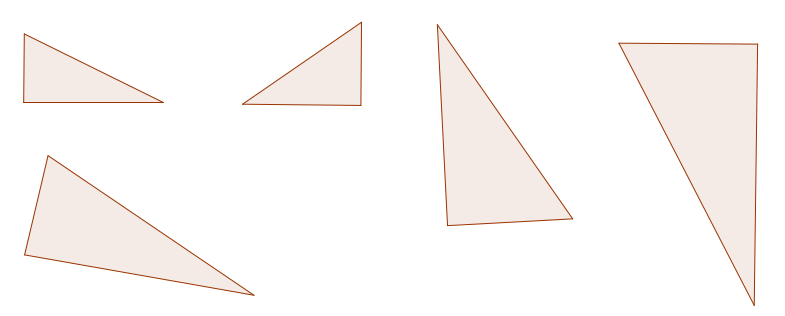
\includegraphics[width=0.6\linewidth]{4x5-pythagore/ex2.png}
\end{figure}

\begin{multicols}{5}
  \begin{enumerate}
  \item[a.] \dotfill 
  \item[b.] \dotfill
  \item[c.] \dotfill 
  \item[d.] \dotfill 
  \item[e.] \dotfill 
  \end{enumerate}
\end{multicols}
\Pointilles[1]

\subsubsection*{Pythagore Rédaction}

\begin{multicols}{2}
\begin{enumerate}
  \item[a.]Soit PVR un triangle rectangle en V tel que : RV = 17,5 cm et RP = 18,5 cm. \\
  \textbf{Calculer la longueur PV.}

  \item[b.]Soit LQF un triangle rectangle en F tel que : QF = 4,8 m et LF = 2 m. \\
  \textbf{Calculer la longueur QL.}

\end{enumerate}
\end{multicols}

\Pointilles[9]

\begin{minipage}[t]{0.65\textwidth}
  \textbf{pb1.} Mario souhaite sauver la princesse Peach en haut d'un château haut de 40m. Pour cela, il jette un grappin par dessus les douves qui ont une longueur de 70m. Calculer la longueur nécessaire du grappin.
  
  \Pointilles[5]
  \end{minipage}
  \begin{minipage}[t]{0.35\textwidth}
  \begin{figure}[H]
    \centering
    \includegraphics[width=0.5\linewidth]{4x5-pythagore/pb1.pdf}
  \end{figure}
\end{minipage}

\newpage

\textit{but princess is in another castle...}

\textbf{pb2.} Mario doit grimper à l'échelle pour aller sauver la princesse. Pour être en sécurité une échelle de 5m doit être écarté de 1,5m du mur. À quelle hauteur maximale peut se trouver la princesse ? \\
\Pointilles[5]

\begin{minipage}[t]{0.65\textwidth}
  \textit{but princess is in another castle...}

  \textbf{pb3.}  \textit{À Pise vers 1200 après J. C. (problème attribué à Léonard de Pise, dit Fibonacci, mathématicien italien   du moyen âge).} \\
  Pour battre Bowser, Mario doit utiliser une lance. Une lance de 6m est posée verticalement le long d’une tour considérée comme perpendiculaire au sol. On éloigne l’extrémité de la lance qui repose sur le sol de 3,6m de la tour. Combien descend l’autre extrémité de la lance le long du mur ?
  \Pointilles[6]
  \end{minipage}
  \begin{minipage}[t]{0.35\textwidth}
  \begin{figure}[H]
    \centering
    \includegraphics[width=0.7\linewidth]{4x5-pythagore/pb3.pdf}
  \end{figure}
\end{minipage}

\Pointilles[2]

\textit{but princess is in another castle...}

\textbf{pb4.}  Mario doit traverser un pont mais celui-ci n'est pas assez solide. Il doit fixer 12 renforts en bois sur les poteaux verticaux qui soutiennent le ponton, comme le montre le dessin. Calculer la longueur d'un renfort puis calculer la longueur totale de tous les renforts nécessaires. 
  
\begin{figure}[H]
  \centering
  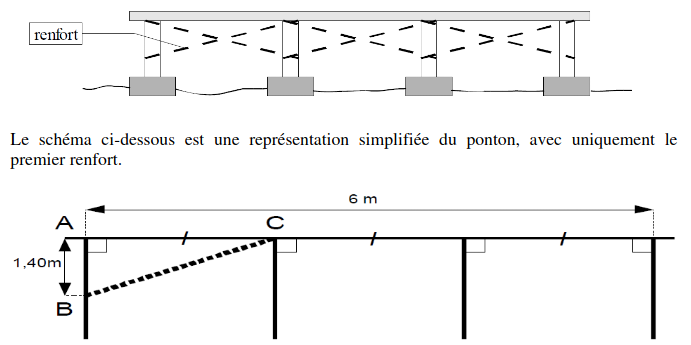
\includegraphics[width=0.6\linewidth]{4x5-pythagore/pb4.png}
\end{figure}
\Pointilles[10]

\end{document}
